\newtheorem{defEdge}{Definition}[section]
\newtheorem{defLoop}[defEdge]{Definition}
%\newtheorem{defInter}[defEdge]{Definition}

\newtheorem{defInv}[defEdge]{Definition}
\newtheorem{defModif}[defEdge]{Definition}

\newtheorem{propPath}{Lemma}[section]

\index{$\execRel^l$}
\section{Representing bytecode programs as control flow graphs}\label{prelim:ctrFlow}

This section will introduce a formalization of an unstructured program in terms of a control flow graph.
The notion of a loop in a bytecode program will be also defined. Note that in the following,
the control flow graph corresponds to a method body. 


%Performing analysis on programs written in  structured languages, is usually easier than performing the same analysis 
%on unstructured programs. In particular, source loops in a method body correspond to a syntactic construction which is not the 
%case for loops in methods on bytecode level. In order to discover a loop in a bytecode program we first need to define 
%what is a bytecode program. Note that in the following, by a  bytecode program we mean a method body.
Recall from Section \ref{clazz} that every method \methodd \ has an array of bytecode instructions \methodd.\body.
%The $k-th$ instruction in the bytecode array $\methodd.\body$ is  denoted with $\methodd.\body[k]$.
 A method entry point instruction is  an instruction at which an execution of a method starts.
 We assume that a method body has exactly one entry point
 and this is the first element in the method body $\methodd.\body[0]$.

 The array of bytecode instructions of a method \methodd \ determine the control flow graph $G( V , \execRel ) $   of method \methodd \ 
in which the vertexes are the instruction indexes of the method body:

$$ V = \{ k \mid   0 \leq k < \methodd.\body.length  \}$$

% The following definition defines the set of edges in the control flow graph.
%\begin{defEdge}[Edge in control flow graph]\label{defEdge}  
%Let us have a control flow graph $G( V , \execRel ) $.
% The set of edges $\execRel$ is a relation between the vertices elements
%$$ \execRel : V * V $$ and is defined  as follows:

 Fig.\ \ref{defEdge} gives the definition of  the execution relation between instructions.
Note first that we rather use the infix notation $j \execRel k$ instead of $(j, k) \in \execRel$.
 Moreover, there is an edge between two vertices's $j$ and  $k$ if they may execute immediately one after another.
 We say that $j$ is a predecessor of $k$ and that  $k$ is a successor of  $j$.
 The definition states the \return \  instruction  does not have successors.
If  $\methodd.\body[j ]$ is the jump instruction $ \ifCond \ k $ then  its successors are the instruction at index $k$   and the instruction at index $j$ in $\methodd.\body$.
From the definition, we also get that every instruction which potentially may throw an exception of type \texttt{Exc}
has as successor the first instruction of the exception handler that may handle the exception type \texttt{Exc}. For instance, a successor
of the instruction $\putfield$ is the exception handler entry point which can handle  the \NullPointerExc \ exception. 
The possible successors of the instruction $\athrow$ are the entry point of any  exception handler  in the method \methodd.
.
% We will also use the notation $\next{j }$ for denoting the successor of   $j$ in a given execution path.
\begin{figure}[ht!]
\begin{frameit}
$$ 
%{\scriptsize  
 \begin{array}{l} 

                    \frac{ \methodd.\body[j] = \nop  } { j \execRel j+1  }
                    \frac{ \methodd.\body[j] = \ifCond \ k  } { j \execRel k  }\\\\
                  
                    \frac{ \methodd.\body[j] = \goto \ k  }{ j \execRel k }\\\\

                    \frac{ \methodd.\body[j] = \putfield \ \findExcHandler{ \NullPointerExc}{j}{\methodd.\excHandlerTable} = k
		     }{ j \execRel k }\\\\

		    \frac{ \methodd.\body[j] = \putfield \ \findExcHandler{ \NullPointerExc}{j}{\methodd.\excHandlerTable} = k
		     }{ j \execRel k  }\\\\ 

		     \frac{ \methodd.\body[j] = \getfield \ \findExcHandler{ \NullPointerExc}{j}{\methodd.\excHandlerTable} = k
		     } { j \execRel k  }\\\\

		     \frac{ \methodd.\body[j] = \arrstore \ \findExcHandler{ \NullPointerExc}{j}{\methodd.\excHandlerTable} = k
		     }{ j \execRel k  }\\\\ 

		     \frac{ \methodd.\body[j] = \arrstore \ \findExcHandler{\ArrIndexOutOfBoundExc}{j}{\methodd.\excHandlerTable} = k
		     }{ j \execRel k  }\\\\ 

		     \frac{ \methodd.\body[j] = \arrload \ \findExcHandler{\NullPointerExc }{j}{\methodd.\excHandlerTable} = k
		     } { j \execRel k  }\\\\ 

                     \frac{ \methodd.\body[j] = \arrload \ \findExcHandler{\ArrIndexOutOfBoundExc }{j}{\methodd.\excHandlerTable} = k
		     }{ j \execRel k  }\\\\ 

		     \frac{ \methodd.\body[j] = \invoke \ \mbox{\rm \texttt{n}}   \ \findExcHandler{\NullPointerExc }{j}{\methodd.\excHandlerTable} = k
		     } { j \execRel k  }\\\\

		     \frac{ \methodd.\body[j] = \invoke \ \mbox{\rm \texttt{n}}  \ 
                                \begin{array}{l}
				     \forall \mbox{\rm\texttt{Exc}}, \exists s , \mbox{\rm \texttt{n}}.\exceptions[s ] = \mbox{\rm\texttt{Exc}} \wedge  \\
		                     \findExcHandler{\mbox{\rm\texttt{Exc}} }{j}{\methodd.\excHandlerTable} = k 
                                \end{array}}{ j \execRel k  }\\\\ 

                     \frac{ \methodd.\body[j] = \athrow  \ \forall \mbox{\rm\texttt{Exc}}, \findExcHandler{\mbox{\rm\texttt{Exc}} }{j}{\methodd.\excHandlerTable} = k}
		    { j \execRel k  }\\\\ 
		   
		    \frac{ \methodd.\body[j] \neq  \goto \  \methodd.\body[j] \neq  \return  \  k = j + 1  } { j \execRel k  }\\\\ 

		   
	
  % \end{array} 
\end{array}%}
$$

\caption{\sc  Execution relation between bytecode instructions in a control flow graph}
\label{defEdge}
\end{frameit}
\end{figure}
%\end{defEdge}




We assume that the control flow graph of every method is reducible, i.e. every loop has exactly one entry point. This actually is admissible
as it is rarely the case that a compiler produce a bytecode with a non reducible control flow graph and the practice shows that even hand written
code is usually reducible. However, there exist algorithms to transform a non reducible control flow graph into a reducible one. 
For more information on program control flow graphs, the curious reader may refer to \cite{ARUCom1986}.
The next definition identifies backlogs in the reducible control flow graph ( intuitively, the edge that goes 
from an instruction in a given loop in the control flow graph to the loop entry)  with the special execution relation $\execRel^l$ as follows:
 
\begin{defLoop}[Backedge Definition]
\label{defLoop}
Assume we have the method \methodd \ with body \methodd.\body \ which determine the control flow graph $G(V, \execRel) $
with entry point $\methodd.\body[0]$.
 In such a graph $G$, we say that $\ins{loopEntry}$ is a loop entry instruction and $\ins{loopEnd}$ is a loop end instruction
 of the same loop if the following conditions hold:
\begin{itemize}
\item for every path $P$ in the control flow graph $P$ from $\methodd.\body[0]$ to  $\ins{loopEnd}$
   % such that  $P~=~\methodd.\body[0] \execRel^{+} \ins{loopEnd}$
     there exists a subpath $subP$ which is a prefix of $P$ and which terminates at $\ins{loopEntry}$  %$subP = \methodd.\body[0] \execRel^{*} \ins{loopEntry}$
          such that $\ins{loopEnd}$ does not belong to   $subP$ %: $\ins{loopEnd} \notin  \ subP  $
%every path in the control flow graph starting at the entry point $\methodd.\body[0]$  that reaches $\ins{loopEnd}$, passes before reaching $\ins{loopEnd}$
% through  $\ins{loopEntry}$ 
\item there is a path in the control flow graph in which $\ins{loopEntry}$  follows immediately after $\ins{loopEnd}$ ( $\ins{loopEnd} \execRel \ins{loopEntry}$)
\end{itemize}
We denote the execution relation between $\ins{loopEnd}$ and  $\ins{loopEntry}$ with \\
$\ins{loopEnd} \execRel^l \ins{loopEntry}$ and we say that $  \execRel^l $  is a loop backedge. 
\end{defLoop}
In  \cite{ARUCom1986},  reducibility is defined in terms of the dominator relation. 
Although  not said explicitly, the first condition in the upper definition corresponds to the dominator relation.%\footnote{we decided to not introduce the standard
%definitions as it has several technical details for the exposition of which we would need more space and which are of not particular interest for the current thesis}.

We illustrate the above definition with the control flow graph of the example from Fig.\ \ref{replaceSrc}.% in Fig. \ref{ctrlflow}.
In the figure, we rather show the execution relation between basic blocks which is a standard notion denoting a sequence of instructions which execute sequentially
and  where only the last one may be a jump and the first may be a target of a jump. 
The black edges represent a sequential execution relation, while dashed edges represent  loop backedge, i.e. the edge which stands for the execution
relation between a final instruction (instruction at index \texttt{18}) in the bytecode cycle and the entry instruction of the cycle (instruction at index \texttt{19}).  
Note that the ``back'' in ``backedge'' stands for  that the control flow goes back to an instruction through which 
the execution path has already passed which does not imply that the orientation of the edge is in a backwards direction in the graphical representation 
of the control flow graph.
% Note that from now on, we are interested in  control flow graphs with the following properties:

% \begin{itemize}
%  \item the control flow graph is reducible
 % \item an exception handler cannot be n
% \end{itemize}
 
\begin{figure}[ht!]
\begin{frameit}
\begin{center}

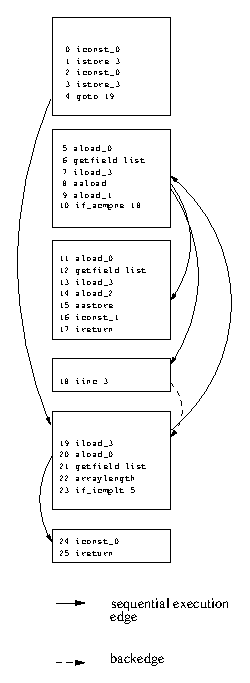
\epsfig{file=figs/bytecode.eps} %, height=5in,  width=1.5in}
\caption{{ \sc The control flow graph of the source program from Fig.\ \ref{replaceSrc}} }
\label{ctrlflow}
\end{center}
\end{frameit}
\end{figure}

%The next lemma states a property about execution paths in a control flow graph that contains backedges. This lemma will be used in the proof of correctness
% of our calculus in section \ref{proof}.
% \begin{propPath} \label{propPath}
% Let's have a control flow graph with an entry point instruction $\methodd.\body[0]$ and two instructions $\ins{loopEntry}$ and  
% $\ins{loopEnd}$ such that  \\
% $\ins{loopEnd}~\execRel^l~\ins{loopEntry}$. If there exists an execution path $P$ from $\methodd.\body[0]$ to  $\ins{loopEnd}$:   $P~=~\methodd.\body[0] \execRel^{+} \ins{loopEnd}$
% then there exists a subpath which is a prefix of $P$  $subP = \methodd.\body[0] \execRel^{*} \ins{loopEntry}$ such that $\ins{loopEnd} \notin  \ subP  $ 
% \end{propPath} 


%Once we have defined what a loop means in a control flow graph, we want also to define what a loop invariant means. 

%\begin{defInv}[Loop Invariant]\label{defInv}
%An invariant is an assertion which accompanies a backedge  in a bytecode control flow graph. Every backedge is accompanied 
%by an invariant. We denote an invariant with $\invariant$. If a backedge  $\execRel^{l}$ is accompanied by an invariant $\invariant$ 
%then $\invariant$ holds in every state in which an execution path passes through  the edge $\execRel^{l}$.    
%\end{defInv}

%We also assume that loop entries are provided with the locations \modifLoop \ that a loop may modify. 
%The interest of having the set of the locations that may be modified by a loop will be seen later when defining the weakest precondition
%predicate transformer.


% \begin{defModif}[Loop Modifies]\label{defModif} Every loop entry instruction $\ins{loopEntry}$ with
%a set of locations $\modifLoop = \{ mod_i \mid  i = 1 .. s\}$ whose meaning is the following: any two states $state_1, state_2 $  in which
% the instruction $ \ins{loopEntry}$ executes agree on local variables and the heap modulo the locations that are in the list \modifLoop.
%We denote the equality between  $state_1, state_2 $   modulo the modifies locations like this 
% $ state_1 =^{\modifLoop } state_2$
%\end{defModif}

